\section*{Problem 4}
For the signals given in Problem 3c) and 3d), use Matlab to plot the truncated 
Fourier series for N = 3, N = 10 and N= 40. (Use subplot to save paper).

\subsection*{Solution}
\begin{enumerate}
\item For problem 3c:
\zcodemat{sources/fapprox3.m}{Approximation of x(t) with Fourier coefficients}

\begin{figure}[H]
\caption{Approximation of x(t) by Xn for N=[3,10,30]}
\centering
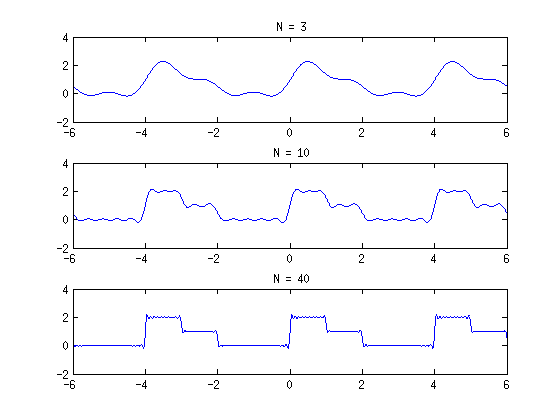
\includegraphics[width=0.8\textwidth]{figs/c1p4.png}
\label{fig:c1p4}
\end{figure} 

\item For problem 3d:
\zcodemat{sources/fapprox4.m}{Approximation of x(t) with Fourier coefficients}

\begin{figure}[H]
\caption{Approximation of x(t) by Xn for N=[3,10,30]}
\centering
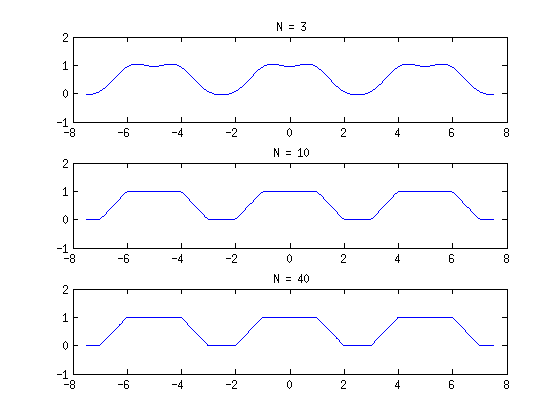
\includegraphics[width=0.8\textwidth]{figs/c1p4b.png}
\label{fig:c1p4}
\end{figure} 


\end{enumerate} 
